Сервис был написан для:
\begin{itemize} 
\item проверки корректности работы платформы;
\item выявление возможных проблем, которые могут произойти на соревнованиях;
\item проведения тренировочной игры.
\end{itemize}

Сервис писался на языке Python с использованием микрофреймворка Flask.

Тестирование платформы заключалось в тестировании следующий функций:
\begin{itemize} 
\item Работа чекера (методы check, get, put);
\item Работа модуля сдачи флагов.
\end{itemize}

Смысл сервиса состоит в том, что в веб-приложении существует возможность добавления и удаления "to do" записей (задачи для выполнения). Также есть функции регистрации и авторизации, т.е. каждый пользователь видит только свои "to do".

Сервис содержит несколько уязвимостей:
\begin{itemize} 
\item backdoor, с проверкой cookies;
\item внедрение SQL кода в cookies (' OR '1'='1);
\item внедрение SQL запроса в записи "to do" (подмена владельца записи "to do").
\end{itemize}

Ниже приведен скриншот работы сервиса (Рисунок 7.2).
\begin{figure}[ht!]
\center{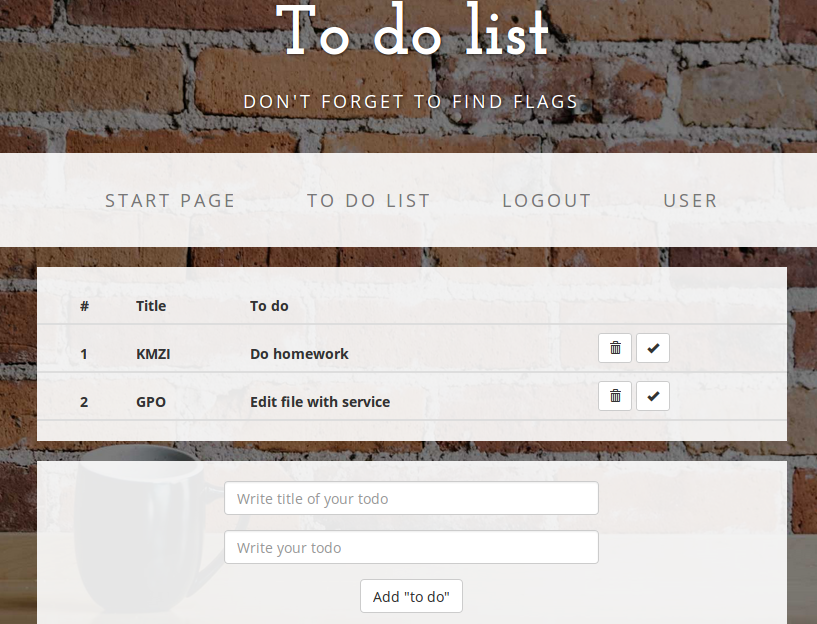
\includegraphics[width=0.8\linewidth]{eco/images/timur_t.png}}
\caption{Сервис todolist}
\end{figure}